\documentclass[../thesis.tex]{subfiles}
\graphicspath{{\subfix{figs/multiling/}}}
\addbibresource{biblio.bib}
\begin{document}

\chapter{Capturing the diversity of multilingual societies}
\label{ch:multiling}

\epigraph{
  To be rooted is perhaps the most important and least recognized need of the
  human soul. It is one of the hardest to define.
}{
  \epigraphcite{WeilNeedRoots2002}
}

Much of the work presented in this chapter is included in an article entitled
\citetitle{LoufCapturingDiversity2021}, that was previously published by the author of
this thesis with Jos\'{e} J. Ramasco and David S\'{a}nchez
\cite{LoufCapturingDiversity2021}.
\\

The research presented in this chapter is concerned with the study of languages in
contact, that is how different languages interact with one another, which emerged a few
decades ago as a hot topic when linguists realised that the world may be facing a mass
extinction of languages
\cite{KraussWorldLanguages1992,GrenobleEndangeredLanguages1998,CrystalLanguageDeath2000}.
As we pointed out in \cref{sec:lang_as_commodity}, there is a great cultural wealth
embedded in these endangered languages, and its loss would be irreversible. Hence the
need to understand what mechanisms drive shifts from one language to another.

Modelling language shift has been the subject of much research in the last decades
\cite{CastellanoStatisticalPhysics2009,BoissonneaultSystematicInterdisciplinary2021},
which employed various approaches such as the formulation of evolution equations based
on ecological models
\cite{MiraInterlinguisticSimilarity2005,PinascoCoexistenceLanguages2006,KandlerEcologicalModels2008,SoleDiversityCompetition2010,HeinsaluRoleBilinguals2014},
of reaction-diffusion equations
\cite{KandlerDemographyLanguage2009,PatriarcaInfluenceGeography2009,IsernLanguageExtinction2014,ProchazkaQuantifyingDriving2017},
or approaches within the framework of agent-based modelling
\cite{CastelloOrderingDynamics2006,MinettModellingEndangered2008,CaridiSchellingvoterModel2013,ProchazkaQuantifyingDriving2017}.
While global evolution equations determine how the proportions of each language group
will evolve in a system, \acp{ABM} describe the shifting mechanisms on an individual
level, as they provide probabilities to switch to another language group. These
transition probabilities depend on the linguistic environment of the individual,
environment which may be defined in many ways.
% Different networks of interactions can be introduced, ranging from the simplest
% (fully-connected networks) to more realistic but less tractable ones (like a
% real-world social network). The former lend themselves easily to mathematical analysis
% as they can be equivalently written in terms of global evolution equations for large
% population sizes. As a result, models based on global evolution equations are a subset
% of the more general, agent-based ones. Moreover,
As explained in \cref{sec:method_theoretical_models}, \acp{ABM} allow to freely define a
linguistic environment, and can thus enable us to assess the impact of the social
structure on the language dynamics. That is why in this chapter we will formulate
existing models and a new proposal of ours in the framework of \acp{ABM}, before showing
the strength of our proposal in both completely interconnected populations and in a
metapopulation framework incorporating the mobility of individuals. We will here turn to
slightly more complex models than one as simple as the Abrams-Strogatz model, which
simply considers the possibility of two monolingual states.

Indeed, the existence of around \SI{6000}{} spoken languages in 200 nations implies that
multilingualism is a pervasive phenomenon worldwide. In almost every country, the
presence of more than one language naturally leads to speech communities of different
sizes. A common situation is that many individuals belonging to these communities use
two or more languages independently of the official status and the educational
prevalence of those languages. The extent and role of bilingualism is hence a difficult
subject. Multiple modelling attempts have been made in that direction
\cite{CastelloOrderingDynamics2006,PatriarcaInfluenceGeography2009,PatriarcaModelingTwolanguage2012,VazquezAgentBased2010}.
In these models, agents can be in a third state AB through which they have to pass to
switch from being monolingual in a language to another. Apart from
\cite{ProchazkaQuantifyingDriving2017} which relied on census data, none of the
aforementioned models have been tested against real-world spatial distributions of
speakers, as they were rather implemented in fully-connected populations or in toy
models, like lattices or random networks. This is a shortcoming we will address here.

Speech communities are distributed in regions which are heterogeneous, and even
discontinuous when their boundaries cannot be arranged into a single closed curve. This
spatial component cannot be neglected in the study of language dynamics, as the
sociolinguistic environment in which individuals interact is of paramount importance for
the dynamics. That is why this work also seeks to obtain and analyse the spatial
distribution of languages in order to evaluate the models. As data on language use with
a fine spatial resolution and large sample sizes are hard to come by using the
traditional sources mentioned in \cref{sec:method_trad_data}, we rather strive to
extract these spatial distributions from Twitter data.

In this chapter, we therefore present results obtained through a combination of a
\graffito{Almost all data analyses, simulations and plots were made using Python code, freely available on GitHub \cite{LoufMultilingtwitter2022}.}
large-scale empirical study of the spatial distribution of languages with metapopulation
modelling.
In \cref{sec:multiling_data}, we show empirically that multilingual societies
are characterised by different spatial patterns in the populations of monolinguals and
bilinguals, encompassing fully mixed states and segregated distributions with a clear
linguistic boundary. As the existing \acp{ABM} are not able to explain the range of
spatial mixing observed, we introduce in \cref{sec:multiling_models} a model able to
capture the diversity seen in the data. The model also shows how the preference of
bilinguals and the ease of learning a language have their importance for the coexistence
of languages. Finally, we present a brief discussion of all the results presented in
this chapter in \cref{sec:multiling_discussion}.



\section{A diversity of multilingual societies?}
\label{sec:multiling_data}
As said above, multilingual societies are numerous and thus susceptible to display
distinct features. These differences, however, need to be observed and, ideally,
quantified, to truly describe the diversity of these societies. Given the very few
regions and countries where censuses gather data on language use at a fine enough
spatial scale, we choose here to turn to Twitter as an alternative data source.
Nonetheless, our analysis can equally be applied to data from surveys and census where
available.


\subsection{Twitter data analysis}
As already mentioned in \cref{sec:methods_twitter}, Twitter has good potential as a data
source to extract spatial distributions of language use. Here, we are not so much
interested in language distributions fitting perfectly what exists in the offline world,
but rather in the kind of distributions we may encounter. Despite all the biases
introduced by the differences of usage of Twitter across the population mentioned in
\cref{sec:twitter_biases}, it could hence still provide valuable insights for regions in
which close to no other data are available. Then to obtain spatial distributions of
languages, we selected 16 countries and regions in which there was potential to gather
sufficient statistics for multilingual communities (see the list in
\cref{tab:region_counts}), and analysed hundreds of millions of geotagged tweets sent
from them from early 2015 to the end of 2019.

A regular grid was laid over each area of interest, dividing them in square cells (see
for instance the grids laid over Belgium and Catalonia in \cref{fig:cat_be_maps}). The
choice of the size of the cells is critical, as it defines the bins of the spatial
distributions that we are studying. There are two limits to the cell size. First is an
upper one, because if too many users are aggregated, we may smooth out relevant
geographical variations in the languages' distributions. The second is a lower one due
to the nature of the geolocation data at hand: the Twitter places data described in
\cref{sec:method_geoloc}. The typical size of places varies between countries, as for
instance cities in America are typically more extended than in Europe. Considering these
two constraints, we thus have to choose cell sizes carefully for each region considered.
Usually, a range of cell sizes is acceptable, and although we choose to show only one in
\cref{fig:cat_be_maps} for instance, our analysis can also be carried out for other
sizes. We will thus show later the robustness of our metrics against cell size changes. 

After thoroughly cleaning and analysing the collected tweets, as described in
\cref{sec:methods_twitter}, we obtain a sample of local Twitter users to which a cell
of residence and their frequency of usage of different languages. As a user may
occasionally tweet in a language they do not speak by way of quoting someone else or
using a translator, we do not keep all of them. We set that at least \SI{10}{\percent}
or 5 of the tweets of a user must be in a certain language to consider them a speaker in
this language. 

Out of hundreds of millions of geotagged tweets posted over a 4-year range, we thus
obtain counts of local users by language group by cell in our 16 regions of interest.
These aggregated data have been deposited on figshare
\cite{LoufSpatialDistributions2021}.

% The data about the knowledge of official languages (English or French or both) by
% census subdivisions in Quebec were obtained from the 2016 Canadian
% census\footnote{\href{https://www12.statcan.gc.ca/census-recensement/2016/dp-pd/dt-td/Rp-eng.cfm?TABID=2&LANG=E&A=R&APATH=3&DETAIL=0&DIM=0&FL=A&FREE=0&GC=01&GL=-1&GID=1159582&GK=1&GRP=1&O=D&PID=110461&PRID=10&PTYPE=109445&S=0&SHOWALL=0&SUB=0&Temporal=2016&THEME=118&VID=0&VNAMEE=&VNAMEF=&D1=0&D2=0&D3=0&D4=0&D5=0&D6=0}{\texttt{https://www12.statcan.gc.ca/census-recensement/2016/dp-pd/dt-td/Index-eng.cfm}}}.


\subsection{Defining pertinent metrics}
Before introducing any metric, let us specify our definition of language groups. First,
we focus only on the languages considered to be local in the area under consideration.
For instance, the use of English is widespread on Twitter, but we do not register those
tweets unless English is one of the local languages (e.g., in Canada or Malaysia). An individual can naturally be in a monolingual or
in a multilingual group if they fulfil the conditions given above in respectively one and more than
one language. The groups defined here are mutually exclusive: each user must be in one
of the monolingual and multilingual groups that are possible to form with the given set
of local languages. For the purposes of our work, we consider language as a social
phenomenon. Thus, we do not take into account the individual proficiency, which is
indeed interesting in other fields of study \cite{BakerFoundationsBilingual1997}, but
instead observe the language production of a speech community defined inside every cell,
based on their use of one or more languages. Thereafter, we will talk of $L$-speakers
instead of ``individuals who belong to the $L$-group'' for the sake of brevity.

Starting from the counts $N_{L,i}$ of $L$-speakers residing in cell $i$ obtained from
the data, we wish to gain insights on the spatial distributions of language use. To do
so we need to define a few basic metrics:
\begin{itemize}
  \item concentration in cell $i$ of $L$-speakers:
    \begin{equation}
    \label{eq:def_conc}
          c_{L,i} = \frac{N_{L,i}}{N_L},
    \end{equation}
  \item proportion of $L$-speakers in $i$'s population:
    \begin{equation}
    \label{eq:def_prop}
          p_{L,i} = \frac{N_{L,i}}{N_i},
    \end{equation}
\end{itemize}
where $N_L = \sum_i N_{L, i}$ are all the users classified as $L$-speakers in the country or region
considered, and $N_i = \sum_L N_{L, i}$ is the population of Twitter users residing in cell $i$ speaking
any of the local languages. As in \cite{MocanuTwitterBabel2013}, we can define the
polarisation of a language A for every cell $i$ in a bilingual system with languages A
and B as 
\begin{equation}
\label{eq:def_polar}
  \theta_{A, i} = \frac{1}{2} (1 + p_{A,i} - p_{B,i}). 
\end{equation}
The polarisation vanishes when there are only B monolinguals and goes to $1$ when there
are only A monolinguals. It takes the neutral value of $0.5$ when there are as many
A-speakers as B-speakers. It also takes this value when there are only bilinguals, as
the proportion of bilingual does not impact this metric and we would then have no
A-speakers and B-speakers --- in the sense given above. We will use this metric in
bilingual regions as an indicator of the mixing at the cell level. 

\begin{figure*}[p!]
  \centering
  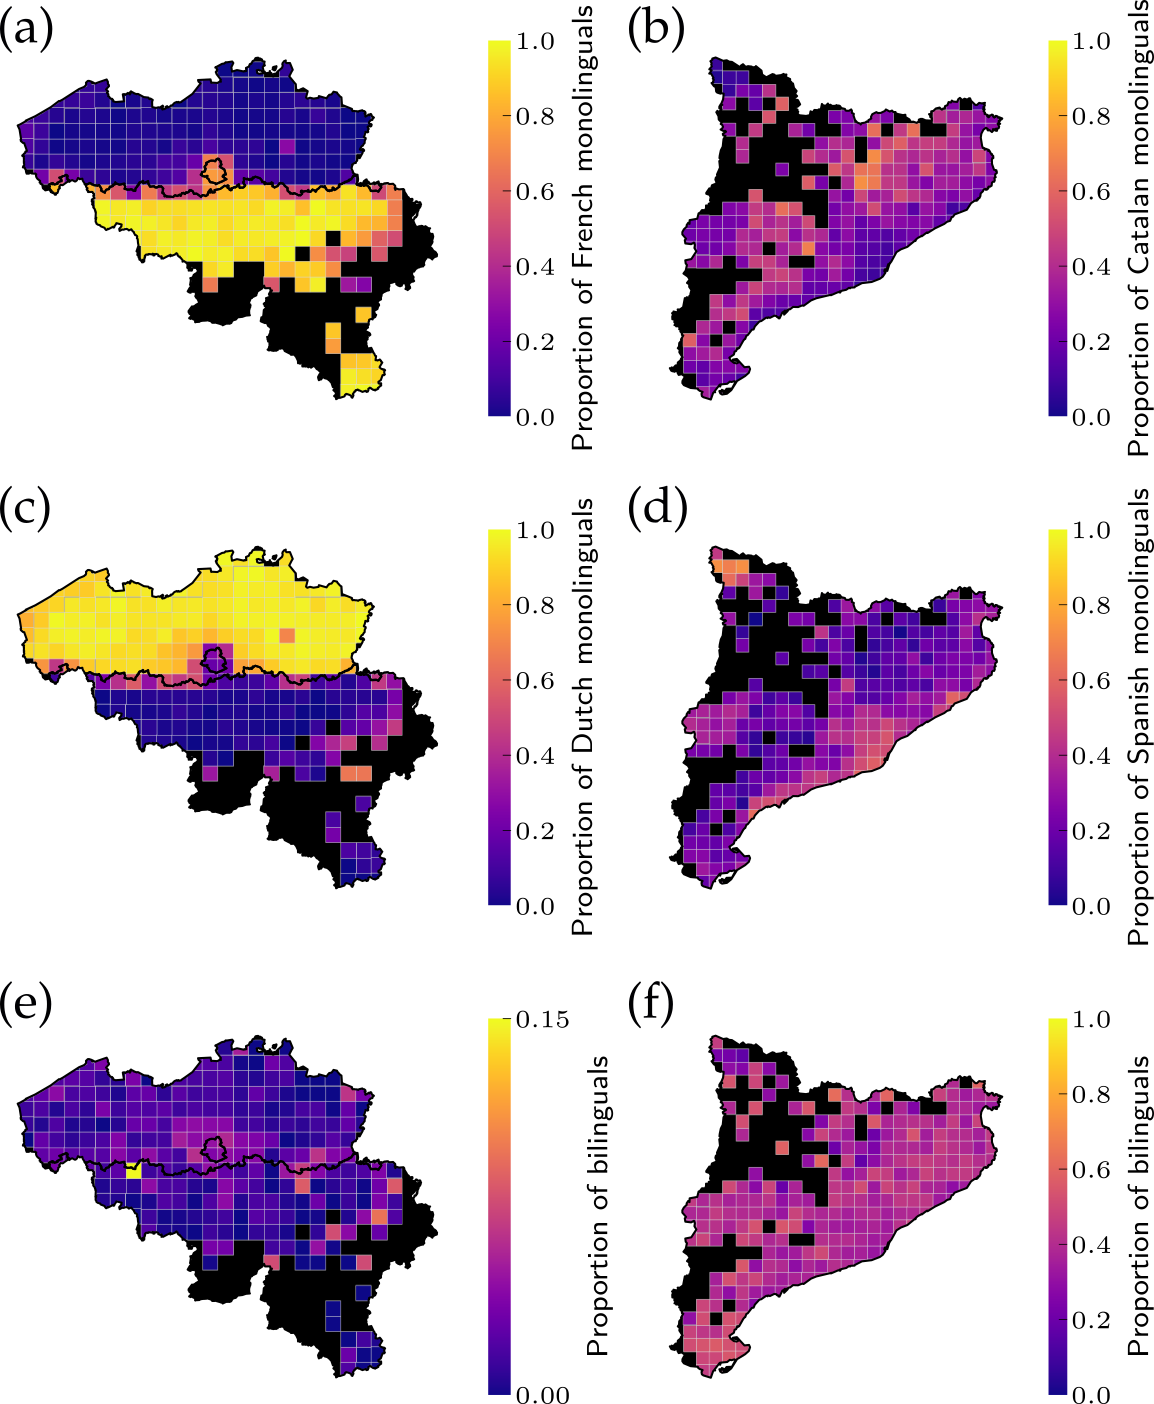
\includegraphics{cat_be_maps.png}
  \caption{Paradigmatic examples illustrating the diversity of multilingual societies.
  For each cell of $10 \times 10 \, \si{\kilo \meter \squared}$, the proportions
  $p_{L,i}$ of monolinguals in (a) French, (b) Catalan, (c) Dutch and (d) Spanish in
  Belgium (left) and Catalonia (right) are shown. The maps (e) and (f) show the
  proportion of bilinguals (note the different scale needed in (e)). In the case of
  Belgium, the border between Flanders (North) and Wallonia (South) is drawn, and the
  Brussels Region too. In black are cells in which fewer than 10 Twitter users speaking
  a local language were found to reside, consequently discarded for the insufficient
  statistics. A clear separation of language groups is visible in Belgium following the
  linguistic regions, displaying mixing mainly around the border and in Brussels, while
  mixing in Catalonia is much more widespread, with a slight difference between the
  countryside and the large cities of the coast (East).}
  \label{fig:cat_be_maps}
\end{figure*}

Building further upon proportions and concentrations, we want to be able to measure the
spatial mixing of language groups, or inversely, their spatial segregation. We define
segregation as the difference in how individuals of a given group are spatially
distributed compared to the whole population. Segregation is thus conceptualised as the
departure from a baseline, the unsegregated scenario, in which regardless of the group
an individual belongs to, they would be distributed according to the whole population's
distribution. Explicitly, the concentrations corresponding to this baseline, or null
model, are
\begin{equation}
  \label{eq:cell_concentrations}
  c_i = N_i / N.
\end{equation}
To quantify language mixing, we would then like to measure a
distance between the spatial distribution of a given language group and that of the
whole population.

To this end, at a full country or region scale, we employ the so-called \ac{EMD}. This
metric allows us to quantify the discrepancy between two distributions embedded in a
metric space of any number of dimensions. It has mainly been used within the field of
computer vision \cite{RubnerMetricDistributions1998}, and it was shown to be a proper
distance (in the metric sense) between probability distributions
\cite{LevinaEarthMover2001}. Here, we consider the distributions defined by the
signatures $P = \{ (i, c_i) \}$ and $Q_L = \{ (i, c_{L,i}) \}$. We then define
$\text{EMD}_L$ as 
\begin{equation}
\label{eq:emd_def}
  \text{EMD}_L \equiv \text{EMD}(P, Q_L) = \sum_{i,j} \hat{f}_{ij} d_{ij}\,,
\end{equation}
with $d_{ij}$ the distances between cells $i$ and $j$, and $\hat{f}_{ij}$ the optimal
flows to reshape $P$ into $Q_L$, obtained by minimizing $\sum_{i,j} f_{ij} d_{ij}$ under
the following constraints:
\begin{equation}
  \left\{
  \begin{aligned}
    f_{ij} & \geq 0, \forall \, i,j \\
    \sum_j f_{ij} & = c_{L,i}, \forall \, i \\
    \sum_i f_{ij} & = c_j, \forall \, j \\
    \sum_{i} \sum_j f_{ij} & = \sum_i c_{L,i} = \sum_j c_j = 1
  \end{aligned}
  \right.
\end{equation}
where $c_i$ and $c_{L,i}$ are the concentrations of the population and $L$-speakers in
every cell $i$, as defined in \cref{eq:cell_concentrations} and \cref{eq:def_conc}.
$\text{EMD}_L$ quantifies thus the distance between the concentration distributions of
$L$-speakers and of the whole population, as needed. The computation of the \ac{EMD} was
implemented with \cite{FlamaryPOTPython2021}, which uses the method of
\cite{BonneelDisplacementInterpolation2011}. However, in its raw form, it is dependent
on the spatial scale of the system considered. Hence the need for a normalisation factor
$k_\text{EMD}$ in order to enable comparisons between regions of different sizes. The
first, obvious choice for $k_\text{EMD}$ would be the maximum distance between two cells
of the region. However, such a choice would neglect the disparities of population
density existing between different regions. The factor would be very high in Quebec, for
instance, since the geographical scales are large even though its northern part is
scarcely populated. This is why we choose instead the average distance between
individuals:
\begin{equation}
  k_\text{EMD} = \frac{\sum_i \sum_j N_i N_j d_{ij} }{\left( \sum_k N_k \right)^2}.
\end{equation}
Our final metric is then the normalised version of the \ac{EMD}, the \acf{EMR}, defined
as:
\begin{equation}
  \label{eq:emr_def}
  \text{EMR}_L = \frac{\text{EMD}_L}{k_\text{EMD}} .
\end{equation}
The \ac{EMR} is a global parameter. The higher it is, the more segregated a linguistic
community. On the contrary, if the \ac{EMR} is close to zero this community is
distributed according to the total population and the mixing is complete. Seeing the
relatively low counts of users found in some language groups, one may wonder whether
such samples may yield reliable measures of segregation through the \ac{EMR}. Therefore,
to determine whether the measure of the \ac{EMR} for a group can be deemed reliable, we
first set a hard minimum of 50 users detected in that group. Then, we order the cells by
descending concentration of the whole population, and take as group count threshold the
inverse of the concentration in the cell corresponding to the $90^\textrm{th}$
percentile of the cumulative distribution. This way, the sample we have can be expected
to have been sufficient to populate significant cells. However, this threshold may not
be passed for a minority group localised in low-density areas, while we may still have a
sufficient sample relatively to its actual size. For this reason, we also test whether
the \ac{EMR} calculation is robust to bootstrap resampling, as we generate 50 samples
from the concentration distribution of this group, calculate the \ac{EMR} each time, and
if the relative standard deviation of these is below \SI{10}{\percent}, we consider the
measured \ac{EMR} of the group to be reliable. We have thus determined that the \ac{EMR}
calculated for the bilinguals in Cyprus, all the multilingual groups in Luxembourg and
the trilinguals in Switzerland were not reliable.


\subsection{Empirical results}
We propose a first visualisation of the collected data in \cref{fig:cat_be_maps}(a)-(d),
where the proportions of monolinguals in Dutch and French, Catalan and Spanish, are
displayed for Belgium and Catalonia, respectively. The cell size is here of $10 \times
10 \, \si{\kilo \meter \squared}$. The maps already show two configurations that
frequently appear across the world in multilingual societies: either a marked boundary
between mostly monolingual domains (Belgium) or high mixing in every cell with local
coexistence (Catalonia). The population of bilingual users concentrates in the border in
the first case (especially in the region around Brussels and in the southern border with
Luxembourg), and it is widespread in the second (\cref{fig:cat_be_maps}(e)-(f)).

The results are summarised in \cref{fig:EMR_countries}(a)-(b), which presents the ranges
of values reached by the \ac{EMR} of respectively the monolingual and multilingual
groups in 14 of our 16 regions of interest.
\begin{figure}[b!]
  \centering
  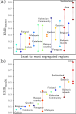
\includegraphics{EMR_countries}
  \caption{\acp{EMR} of the (a) monolingual and (b) multilingual groups of multilingual
  regions of interest, ranked left to right by increasing average of the $y$-axis
  values. In (b), the point for trilinguals in Switzerland is not displayed because its
  value was deemed unreliable. All values of the \ac{EMR} shown here, as well as those
  that we discarded are given in \cref{tab:table_multiling_charac}. A rich diversity of
  mixing patterns is shown, beyond the two paradigmatic cases of Catalonia and Belgium.}
  \label{fig:EMR_countries}
\end{figure}
As mentioned previously, we filtered out regions where we deem not sufficient the
statistics gathered from Twitter. A wide diversity of situations can be observed.
Multilingual societies may have rather balanced monolingual groups separated by a
clear-cut border, which have thus high but quite similar \ac{EMR} values, like in
Belgium and Switzerland. One can also see unbalanced situations where one language is
spoken by the majority, and has thus a much lower \ac{EMR} than the monolinguals and
multilinguals of other smaller, isolated languages. This is for example the case on the
island of Java, where Indonesian is widespread, and Javanese and Sundanese are more
localised. Multilinguals may also be mixing well in the whole population, like the
bilinguals in Galicia and Catalonia. These groups can thus be of completely different
natures from one region to another, from sustaining a minority language while being
spatially mixed or isolated, to standing at the border between monolingual communities.
To demonstrate the robustness of the \ac{EMR} as a metric on spatial distributions and
the soundness of our choices of cell sizes, we show in
\cref{fig:EMR_cell_size_invariance} that the \ac{EMR} is cell-size-invariant for
reasonable choices of cell sizes.
\begin{figure}[h!]
  \centering
  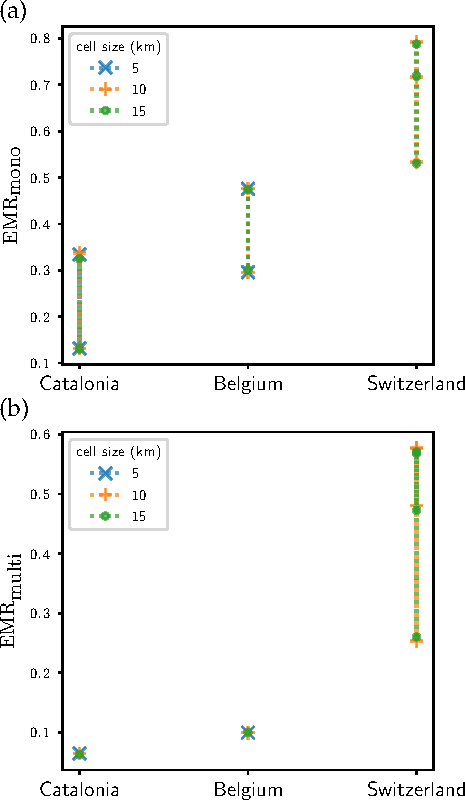
\includegraphics{EMR_cell_size_invariance}
  \caption{Robustness of the \ac{EMR} with regard to the choice of cell size. For cell
  sizes ranging from $5 \times 5 \, \si{\kilo \meter \squared}$ to $15 \times 15 \,
  \si{\kilo \meter \squared}$ in Catalonia, Belgium and Switzerland, the values of the
  \ac{EMR} (a) between the monolinguals in each language and the whole population, and
  (b) between the multilinguals and the whole population are shown.}
  \label{fig:EMR_cell_size_invariance}
\end{figure}

All metrics introduced in this section can be computed using similar data taken from
other sources to evaluate the spatial mixing of languages.
% Although data on language use on a fine enough spatial scale are difficult to find, it
% can, for instance, be obtained for Quebec from the Canadian census of 2016. Maps
% equivalent to the ones of \cref{fig:cat_be_maps} are shown using both data from the
% census and from Twitter for Quebec in the SI Figs. S13 and S14 \cite{supp}. Similar
% mixing patterns can be observed from both data sources.



\section{Models capturing diversity}
\label{sec:multiling_models}
As language use in a society only sees significant changes on a timescale of generations
\cite{LabovSociolinguisticPatterns1973}, the maps obtained from Twitter are only
snapshots of the situation around the years 2015 to 2019. In other words, it gives a
synchronic view. We do not have access to data providing the longitudinal evolution
(diachronic framework), while the models at hand describe the dynamics of the system.
Still, since some of the multilingual societies we study have had the same kind of
spatial pattern of language coexistence for generations (Belgium with a separation and
Catalonia with mixing), it is natural to ask whether these states are stable solutions
of a model describing language competition. We will check, in the first place, if the
existing models meet the basic requirement of reaching the observed stable states.
Crucially, if they do not fulfil it, the underlying mechanisms of language shift are not
therein fully captured, missing a significant element that could be key to language
preservation.


\subsection{Previous models}
The individuals in a population can be in states representing their use of one or
several languages. Under this framework, the dynamics are governed by the permitted
transitions between states and their corresponding probabilities of occurring.
\Cref{fig:multiling_models_diagram} displays the states: monolingual in A and B, and bilingual AB,
with the associated transition probabilities in two previous models and in our proposal.
We denote $p_{\text{A}}$ and $p_{\text{B}}$ the proportions of monolinguals in A and B,
respectively, and $p_{\text{AB}}$ the proportion of bilinguals. These satisfy the
equality $p_{\text{A}} + p_{\text{B}} + p_{\text{AB}} = 1$. Within this notation, a
state of coexistence is a state in which the two languages remain spoken, which
corresponds to either $p_{\text{AB}} > 0$, or $p_{\text{A}} > 0$ and $p_{\text{B}} > 0$.
Extinction of A (B), for instance, corresponds to $p_{\text{A}} = p_{\text{AB}} = 0$
($p_{\text{B}} = p_{\text{AB}} = 0$).
\begin{figure}
\centering
  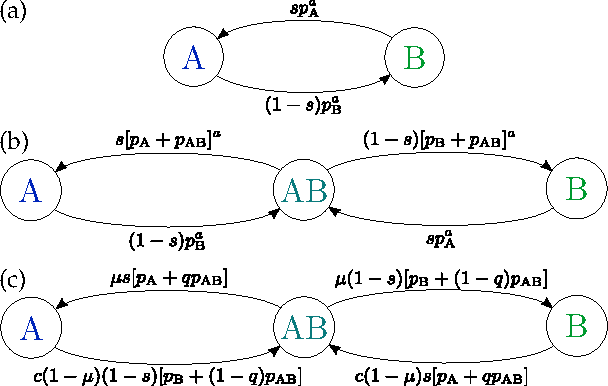
\includegraphics{models_diagram}
  \caption{Diagrams of the models presented in the text, showing the transition
  probabilities from one state to another. (a) Abrams-Strogatz model from
  \cite{AbramsModellingDynamics2003}. (b) Bilinguals model from
  \cite{CastelloOrderingDynamics2006}. (c) Our model of bilinguals including both
  their preference and the ease to learn the other language (see
  \cref{eq:bipref_model}).}
  \label{fig:multiling_models_diagram}
\end{figure}

The first model to mention is the one introduced in \cite{AbramsModellingDynamics2003}
by Abrams and Strogatz (\cref{fig:multiling_models_diagram}(a)). We already briefly introduced the
model in \cref{sec:method_theoretical_models}, but let us give a brief reminder of
notation and features of the model. The model only contains monolinguals, who can change
their languages with a probability that depends on the proportion of speakers of the
other language to an exponent $a$ (called volatility), which controls if the dependence
on the proportion of the other language group is linear ($a = 1$), sublinear ($a<1$) or
superlinear ($a>1$). Besides, they also include a parameter $s$ between zero and one,
which stands for the prestige of the language A. If $s$ is close to one, all the
individuals will forget B and start to speak A alone.
% Set in a single population and in mean-field, this model was shown to fit historical
% data of the decline of minority languages in \cite{AbramsModellingDynamics2003}.
The model was thoroughly analysed in \cite{VazquezAgentBased2010}, where it was first
shown that its stable state is extinction of one language for $a \ge 1$, and coexistence
for $a < 1$, independently of the prestige, as shown previously in
\cref{fig:AS_fc_param_space}.
% In complex contact networks, the coexistence region in the $(s, a)$ space shrinks, as
% not all values of prestige enable coexistence for $a < 1$.
It is important to note that the linear version of the model does not predict
coexistence.    

Later, an extended model with bilinguals was proposed by Castell\'o et al.
\cite{CastelloOrderingDynamics2006} (see \cref{fig:multiling_models_diagram}(b)). The transitions
to lose a language are there related to the proportion of bilinguals besides the
monolinguals of the other side. The idea is that since A can be spoken to both A and AB
individuals, the utility to retain B decreases with an increasing proportion of these
two types of individuals. An analysis of the stable states of this bilinguals model
performed in \cite{VazquezAgentBased2010} shows that the coexistence only occurs if $a <
1$ and that the area of parameters allowing it is reduced compared to the
Abrams-Strogatz model. Again, the linear ($a = 1$) version of the model does not allow
for language coexistence.

Several concerns may be raised about these models. The first one is that for languages
with equal prestige ($s = 1/2$) and with equal social pressure (same proportion terms),
learning and forgetting a language is equiprobable, while they result from two
completely different processes. People may inherit a language from their parents, use it
for endogenous communication, and they could be driven to learn a new one for work or
education purposes, which corresponds to exogenous communication. This is a typical
situation of diglossia \cite{FergusonDiglossia1959} with a linguistic functional
specialisation. A difference in prestige favours this process, but losing a language,
especially in the presence of cultural attachment, can be more difficult. In the case of
bilingualism, once someone masters a new language to a bilingual level they will not
forget their first. Besides, it seems reasonable to assume that most of the time, a
language is lost when it is not passed from one generation to the next
\cite{CrystalLanguageDeath2000,PortesPluribusUnum1998}. A second concern we raise here
is that both models only find stable coexistence in a nonlinear configuration, when $a <
1$. These values of $a$ imply easier transitions overall, and thus that coexistence is
favoured when speakers are more loosely attached to their spoken languages. It is
however hard to argue that French speakers in Quebec or Catalan speakers in Catalonia
are loosely attached to these languages. This nonlinearity is hence hard to explain from
a practical point of view, and it has the effect of making the transitions less
dependent on the actual proportions of speakers. Thirdly, it is important to note that
the bilingual model of \cref{fig:multiling_models_diagram}(b) is not able to produce a stable
solution in which the bilinguals coexist with monolinguals of a single language.


\subsection{Our model}
Our proposal stems from the realisation of this last point: there are several bilingual
societies where the monolinguals of one language, e.g., B, are virtually extinct (e.g.,
Catalonia, Quebec or the Basque Country). However, the bilinguals continue to use B and
keep it alive for decades if not centuries due to cultural attachment. This ``reservoir
effect'' must be incorporated in models of language shift. The other ingredient that we
will include concerns demographics, in relation with the first concern raised above:
language loss mostly occurs between generations. For this, we get inspiration from the
work of \cite{MinettModellingEndangered2008} that sets a rather generic framework for
models differentiating horizontal and vertical transmission.

We thus first distinguish generational, or vertical, transmission, which corresponds to
the death of a speaker replaced by their offspring. If the speaker was monolingual,
their single language is transmitted. If they were bilingual, one of their two languages
might get lost in the process of transmission. This loss occurs according to the
following transition probability:
\begin{equation}
  P (\text{AB} \rightarrow \text{X}) = \mu \, s_\text{X} \, \left[ p_{\text{X}} + q_\text{X} \, p_{\text{AB}} \right],
\end{equation}
where, as in the other models, $s_\text{X}$ refers to the prestige of language X, which
can be either A or B. The other parameters are $\mu \in [0, 1]$, that is the fixed
probability for an agent to die at each step, present in the model of
\cite{MinettModellingEndangered2008}, and $q_\text{X} \in [0, 1]$, that reflects the
preference of bilinguals to speak X, which has not been considered in previous works. So
bilingual speakers may be more inclined to transmit only language X when it is more
prestigious, preferred by other bilinguals, and more spoken around them.

The second kind of transition is horizontal, it is related to the learning of a new
language by a monolingual in the course of their lives. This transition occurs according
to the following transition probability:
\begin{equation}
  P (\text{X} \rightarrow \text{AB}) = c \, (1 - \mu) \, s_\text{Y} \, \left[ p_\text{Y} + q_\text{Y} \,  p_{\text{AB}} \right],
\end{equation}
where Y is the language other than X, and, critically, $c \in [0, 1]$ is a factor
adjusting the learning rate. The time scales of the learning process and of a
generational change are completely different, hence the need to adjust $(1-\mu)$ by this
factor $c$ here. It depends on the similarity between the two languages and on the
implemented teaching policies. For the sake of simplicity and to avoid the inclusion of
more parameters, we assume that the process is symmetric between learning A when B is
spoken and vice versa. This is not necessarily true in all cases, but it can easily be
solved by splitting $c$ in more parameters for each transition. To translate this
expression of the transition probability into words, a monolingual in X will be more
willing to learn Y as it is easier to learn, more prestigious, preferred by bilinguals,
and more spoken around them.

We define $s$ and $q$ as symmetric around $1/2$, and thus define $s = s_\text{A} = 1 -
s_\text{B}$ and $q = q_\text{A} = 1 - q_\text{B}$. The transitions in our model are
illustrated in \cref{fig:multiling_models_diagram}(c) and we write here below the transition
probabilities that define it:
\begin{equation}
\label{eq:bipref_model}
\left\{
\begin{aligned}
  P (\text{A} \rightarrow \text{AB}) &= c \, (1 - \mu) \, (1-s) \, \left[ p_{\text{B}} + (1-q) \,  p_{\text{AB}} \right] \\
  P (\text{B} \rightarrow \text{AB}) &= c \, (1 - \mu) \, s \, \left[ p_{\text{A}} + q \, p_{\text{AB}} \right] \\
  P (\text{AB} \rightarrow \text{A}) &= \mu \, s \, \left[ p_{\text{A}} + q \, p_{\text{AB}} \right] \\
  P (\text{AB} \rightarrow \text{B}) &= \mu \, (1-s) \, \left[ p_{\text{B}} + (1-q) \, p_{\text{AB}} \right]
\end{aligned}
\right.
\end{equation}
Given the normalisation condition $p_\text{A} + p_\text{B} + p_\text{AB} = 1$, these
transition probabilities can actually be rewritten in terms of, let us say, $p_\text{A}$
and $p_\text{B}$ only. An important aspect of the model is that the use of a language by
bilinguals contributes potentially unequally to the sizes of each language community.
The neutral case occurs when $q = 1/2$ and bilinguals on average contribute equally to
both groups. It is however natural that even if bilinguals are fluent in both languages,
individually they may have a certain preference for one of them and their language use
is not necessarily balanced \cite{RomaineBilingualMultilingual2012}. Even if one of the
two languages is in a minority or suffers from a lack of prestige, appropriate values of
$q$ may maintain it alive. The most extreme example occurs when the monolinguals of B,
for example, are extinct ($p_{\text{B}} = 0$). Still, the use of B by the bilinguals
keeps attracting monolinguals of the group A proportionally to $(1-q)\, p_{\text{AB}}$.

Finally, we chose not to include non-linearities in the model ($a = 1$), as it turned
out not to be necessary to capture the diversity we observed, and it would only add
unnecessary complexity.


\subsection{A single population}
\label{sec:multiling_mean_field}
We first analyse the model \graffito{Figures shown in this section were generated with
Mathematica code, freely available on GitHub \cite{LoufMultilinganalytical2022}.} in the
simplest setting of a single completely interconnected population to determine the
typology of possible solutions. A mean-field approximation yields:
\begin{equation}
  \label{eq:dt_bipref_model}
  \left\{
  \begin{aligned}
    \dv{p_\text{A}}{t} &= (1 - p_\text{A} - p_\text{B}) P (\text{AB} \rightarrow \text{A})
        - p_\text{A} P (\text{A} \rightarrow \text{AB})
    \\
    \dv{p_\text{B}}{t} &= (1 - p_\text{A} - p_\text{B}) P (\text{AB} \rightarrow \text{B})
        - p_\text{B} P (\text{B} \rightarrow \text{AB})
  \end{aligned}
    \right.
\end{equation}
Fixed points are the solutions for which $\dv{p_\text{A}}{t} = \dv{p_\text{B}}{t} = 0$.
The stability of these points is studied by performing a linear perturbation analysis
around them, which requires the calculation of the Jacobian of the linearised equations
and of its eigenvalues. Points for which all the eigenvalues have strictly negative real
parts are stable, while if any eigenvalue's real part is zero or positive the fixed
point is unstable. Stream plots in \cref{fig:stream_plots} show where the model
converges to in three characteristic examples, depending on the model parameters.
\begin{figure}[b!]
  \centering
  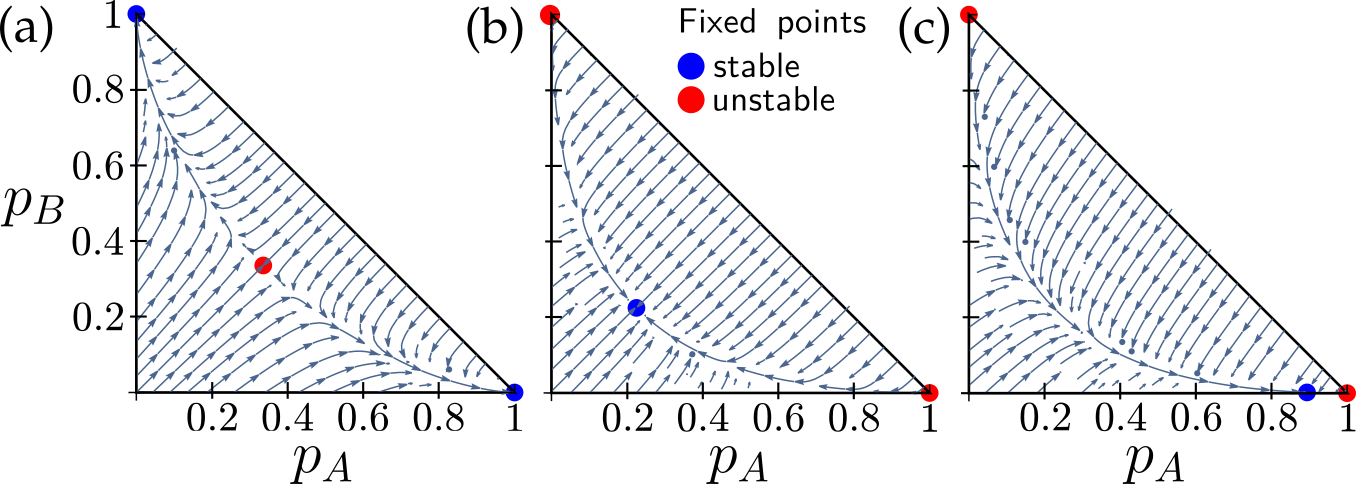
\includegraphics[width=\textwidth]{single_pop_stream_plots.png}
  \caption{Stream plots for the dynamics of two languages according to our model
  described in \cref{eq:bipref_model} set in a well-mixed population. $p_{\text{A}}$
  and $p_{\text{B}}$ denote the proportions of monolinguals in A and B, respectively,
  and the proportion of bilinguals $p_{\text{AB}}$ is such that $p_{\text{A}} +
  p_{\text{B}} + p_{\text{AB}} = 1$. The mortality rate is fixed at $\mu = 0.02$. (a)
  For $s = q = 1/2$ and $c=0.02$, the stable outcome is extinction of one of the two
  languages. (b) For $s = q = 1/2$ and $c = 0.05$, the higher learning rate leads to a
  solution featuring stable coexistence. (c) For $s = 0.57$, $q = 0.45$ and $c =
  0.05$, despite a lower prestige, B survives in a small community of bilinguals as
  it is the preferred language among them.}
  \label{fig:stream_plots}
\end{figure}
In the first one (\cref{fig:stream_plots}(a)), the stable (blue) points lie over the
axis at values 1 and the system has as only solution the extinction of one of the two
languages. In \cref{fig:stream_plots}(b), the stable fixed point falls in the middle of
the diagram and, therefore, the solution is symmetric coexistence with a majority ($\sim
1/2$) of bilinguals. Finally, in \cref{fig:stream_plots}(c), we find a stable fixed
point over the $x$-axis that represents the extinction of monolinguals B but coexistence
between A-monolinguals and bilinguals. Surprisingly enough, this represents the survival
of a less prestigious language within a relatively small bilingual community. These
results show already the flexibility of the model even in a single population.
Remarkably, it does so without introducing extra parameters to fit. Indeed, $\mu$ and
$q$ are both quantities that can be measured in real-world scenarios, as opposed, for
instance, to the inter-linguistic similarity introduced by
\cite{MiraInterlinguisticSimilarity2005} that is, as said explicitly in this work, not
straightforward at all to calculate, and is thus an extra parameter that needs to be fit
to data. Moreover, although it is out of the scope of this work, the parameter $q$ can
naturally be measured on an individual level, which can be used to initialise more
realistic simulations within an \ac{ABM} framework.

We change now the viewpoint from the phase space to the parameter space. In
\cref{fig:coex_region}, we plot the region of parameters where the model converges to
stable coexistence. Since $c$ and $\mu$ act over the stability only in a combined form,
their contributions can be merged into a new variable $r$ defined as
\begin{equation}
  \label{eq:r_def}
  r = \frac{\mu}{c \,(1-\mu)},
\end{equation}
which stands for the ratio between the mortality and learning rates. The
other two parameters, $s$ and $q$, are considered independently. We observe that the
coexistence region expands when $r$ decreases. This means that increasing the ease to
learn one language when knowing the other (with a fixed mortality rate) makes
coexistence more likely. Additionally, coexistence occurs more frequently when both
prestige and bilingual preference are neutral, $s = q = 1/2$, which is expected. When
the prestige of language A is lower than that of B, we find that there exists an optimal
value of $q$ making possible the coexistence, $q^\text{opt} > 1-s$. For $q <
q^\text{opt}$, $A$ is more at risk of extinction whereas for $q > q^\text{opt}$, the
endangered language is $B$. There is thus a balance between prestige and bilingual
preference that enables coexistence.
\begin{figure}[h]
  \centering
  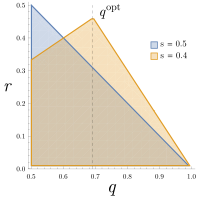
\includegraphics[width=7cm]{single_pop_param_space}
  \caption{Region of the parameter space where the dynamics of our model in a single
  population converge to stable coexistence of languages. We show two 2D cuts of the
  coexistence region in the ($q$, $r$) space for fixed values of $s=0.5, 0.4$, with $r$
  as defined in \cref{eq:r_def}. Lower values of $r$ favour coexistence, as well as a
  neutral prestige and bilingual preference $q$. When $s < 0.5$, coexistence is favoured
  for an optimal value $q^\text{opt} > 1-s$.}
  \label{fig:coex_region}
\end{figure}

This model opens up unique classes of stable solutions: from the extinction of a
language to coexistence when prestige is neutral, but also when it favours one of the
two languages, and even only through a community of bilinguals. However, these analytic
results in a fully-connected population do not suffice, as they do not show if the model
is able to reproduce a case such as Belgium, where in the majority of cells there
remains almost exclusively one language, except on the boundary between the two large
communities. Consequently, we will now analyse the model in a metapopulation framework
to uncover the effect of including space and check whether this pattern can arise.


\subsection{The model in space}
In our context, we would need some information to build the extended model within this
metapopulation framework. The basic ingredients are a spatial division, the population
in each division, the mobility between them and the characteristics of the populations
in terms of language groups. Since we are interested in the phase space of the model, it
is possible to use a completely abstract setting. However, this would require the
generation of reasonable data in terms of population and mobility, while this
information is easily accessible from census data in many countries. Since we wish here
to study the stability of the present, observed state, to make metapopulations interact
with one another we use readily-available commuting data from the census, as commuting
is the backbone of everyday mobility. Some further work could include other kinds of
mobility, like migrations, in order to investigate long-term time evolutions. We have
thus chosen to use census data in Belgium as a benchmark, although it is important to
stress that the intention is not to produce accurate predictions. Alternatively, the
spatial interactions could be estimated from the population data using a model of human
mobility, such as gravity, radiation or distance-kernel-based models
\cite{BarbosaHumanMobility2018,BurridgeSpatialEvolution2017,BurridgeInferringDrivers2021}.

\begin{figure}[hp!]
  \centering
  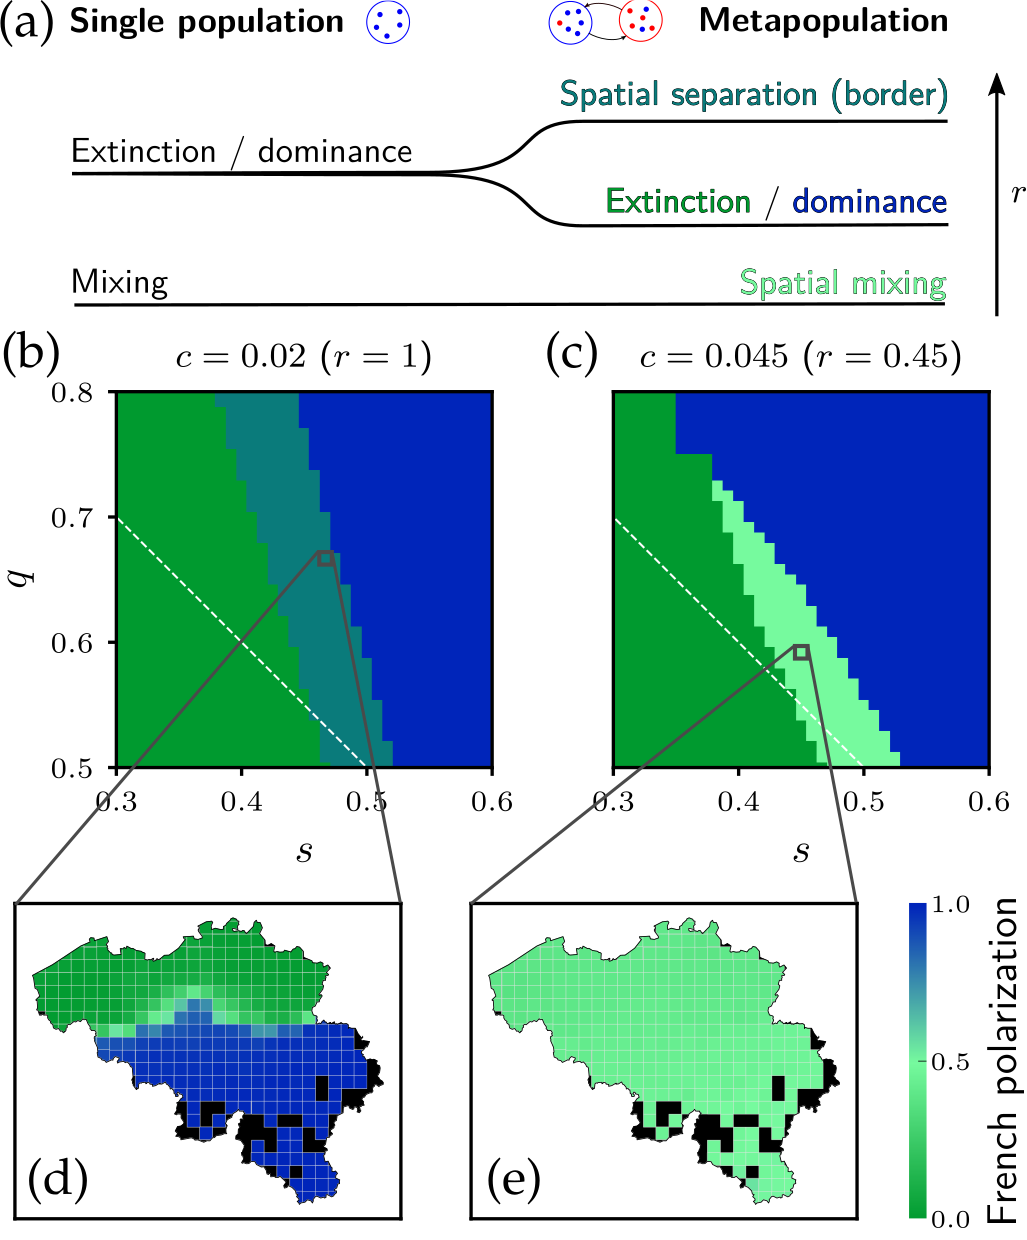
\includegraphics{single_to_metapop_BE.png}
  \caption{Types of stable states of convergence of our model in a metapopulation set
  for Belgium. (a) Diagram illustrating the effect of adding metapopulations in the
  stable states of a single population: the former extinction state bifurcates in full
  extinction and in a boundary-like state with monolinguals separated in space. Larger
  values of $r$ favour homogeneity, either by full extinction or by separation states.
  Below are the regions of the parameter space $(s,q)$ where these stable solutions
  emerge, (b) with $r=1$ and (c) with $r=0.45$. Finally, two maps of the French
  polarisation (A = French and B = Dutch in \cref{eq:def_polar}) show examples of
  states the model converges to, (d) a boundary-like state for $r=1$, $s=0.467$,
  $q=0.667$, and (e) complete mixing for $r=0.45$, $s=0.45$, $q=0.592$. $s$ and $q$ are
  defined as the prestige of and preference for French.}
  \label{fig:single_to_metapop_BE}
\end{figure}

The populations and commuting patterns at the municipality level are thus obtained from
the national census of
2011\footnote{\url{https://statbel.fgov.be/en/open-data/census-2011-matrix-commutes-sex}}.
We implement a mapping process from municipalities to our cells based on area overlap,
similarly to what we described in \cref{sec:method_geoloc}.

Regarding the language groups, since we are mixing commuting data from the census with
data from Twitter, we first have to up-scale the number of individuals we found from
Twitter data to match the number of commuters. Instead of up-scaling uniformly by the
ratio between these two numbers, we choose here to alleviate the socio-demographic
biases that we mentioned in \cref{sec:twitter_biases} through re-scaling factors
$k_{L,i}$, which are different between cells and language groups. The first bias to
address is how users are more urban than average
\cite{MisloveUnderstandingDemographics2011}, which leads us to impose the constraint
$\sum_L k_{L,i} N_{L,i} = N_i^\text{(census)}$. The second one is how language usage is
different on Twitter, because one's audience is wider, potentially more cosmopolitan
than offline \cite{NguyenAudienceUse2015}, and with different demographics
\cite{MisloveUnderstandingDemographics2011}. Hence we want to also re-scale such that
$\sum_i k_{L,i} N_{L,i} = N_L^\text{(census)}$, with $N_L^\text{(census)}$ the global
numbers of $L$-speakers, data which are much more widely available than the counts for
each census tract. By imposing these two constraints, it is assumed that the two biases
are independent: the bias in the choice of language used online is space-independent in
a specific multilingual society, and the over-representation of urban people is
$L$-group-independent. In practice, we fit the values of the upscaling factors $k_{L,
i}$ via \ac{IPF} \cite{DemingLeastSquares1940,FienbergIterativeProcedure1970}.

Once the metapopulation has been initialised, the model can be simulated. As in
\cite{Fernandez-GraciaVoterModel2014}, the day is divided in two parts: the individuals
first start in their residence cells and interact with the local agents following the
rates of \cref{eq:bipref_model}, and then move to their work cells where again they
interact with the local population. The agents encounter thus different environments
characterised by diverse proportions $p_{L,i}$ in the two parts of the day. Even if they
live and work in the same cell, the local population changes from one part of the day to
the next.

In order to analyse the stability of the steady states reached by the extended model, we
derive an approximate master equation for the full metapopulation setting. To this end,
we adapt the methodology described in
\cite{SattenspielStructuredEpidemic1995,BalcanModelingSpatial2010} for epidemiological
models. Our derivations and the resulting equations are given in
\cref{ch:appendix_metapop_equations}. The equations obtained are only approximated, but
since they are analytic we can integrate them and calculate the Jacobian at their fixed
points. To check the consistency of both approaches and that the fixed points of the
dynamics are the same, we also introduce the initial conditions in the master equation,
to then integrate it numerically using a standard Runge-Kutta algorithm. The fixed
points reached by the simulations turn out to be fixed points as well for the equations.
Not only that, all the eigenvalues of the Jacobian at these states have negative real
parts, and they are thus stable fixed points.

To explore the parameter space systematically, we perform a number of simulations until
convergence to a stable state. We show the results for the metapopulation setting of
Belgium in \cref{fig:single_to_metapop_BE} and \cref{fig:metapop_phase_space_all_c}.
Remarkably, a new kind of stable state emerges. While in a single population we had only
two stable configurations: extinction or mixing, here we can find full mixing
(\cref{fig:single_to_metapop_BE}(e)), global extinction and local extinction of a
language in part of the territory leading to a boundary-like state
(\cref{fig:single_to_metapop_BE}(d)). This state of convergence is similar to the
initial conditions, corresponding to the language border we observe today. We have thus
checked that our model, in these conditions, is able to obtain the present state as a
stable solution. A surprising aspect of the results is that decreasing $r$, or in other
words making it easier or more common to learn the other language, does not necessarily
favour coexistence, as shown in \cref{fig:metapop_phase_space_all_c}. Indeed, as $r$
decreases, at one point boundary states become unstable and this may not necessarily
lead to fully mixed states. When $r$ shrinks bilinguals become more numerous on the
boundary, until they expand beyond the boundary and spread bilingualism across the
region. Still, if this happens when $r$ is not low enough, the two languages cannot
coexist and one ends up extinct, as the coexistence region of the parameter space in a
single population shown in \cref{fig:coex_region} may not have been reached. 
\begin{figure}[p]
  \centering
  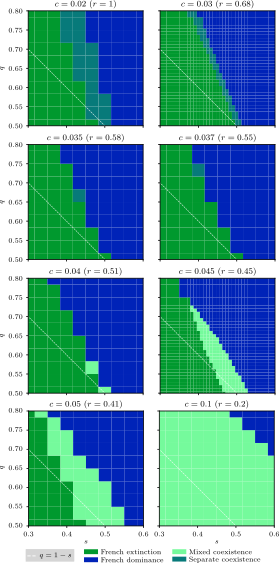
\includegraphics{smaller_metapop_phase_space_all_c}
  \caption{Phase space of the stable states of convergence of our model when iterated
  within our metapopulation framework in Belgium. Colours show the kind of convergence
  state reached for the corresponding set of parameters. A lower learning rate, that is
  a lower value of $c$, favours the separate coexistence of French and Flemish, while a
  higher one favours mixed coexistence. In the transition between the two however,
  coexistence is almost impossible, as the corresponding region in the $(s,q)$ space
  becomes very narrow.
  % Here again, $s$ and $q$ are defined as the prestige of and preference for French
  }
  \label{fig:metapop_phase_space_all_c}
\end{figure}

% We also wished to explore the possibility of having a hybrid state, consisting in an
% area where a minority language survives through bilinguals within an otherwise
% monolingual region. This is the case of Sundanese and Javanese in Java for instance. We
% initialised a hypothetical population in Belgium, with only monolinguals in Dutch,
% except in a pocket of cells in the South of the country, where there are only
% bilinguals. The latter were attached a $q = 0.62$, while $q = 0.5$ for the rest.
% Iterating the model yields a stable solution similar to this initial state, with a mix
% of bilinguals and Dutch monolinguals in the pocket, and only Dutch monolinguals
% elsewhere.
% TODO: include? (see SI Fig. S15 \cite{supp}).


\subsection{Dynamics in the parameters}
\begin{figure}
  \centering
  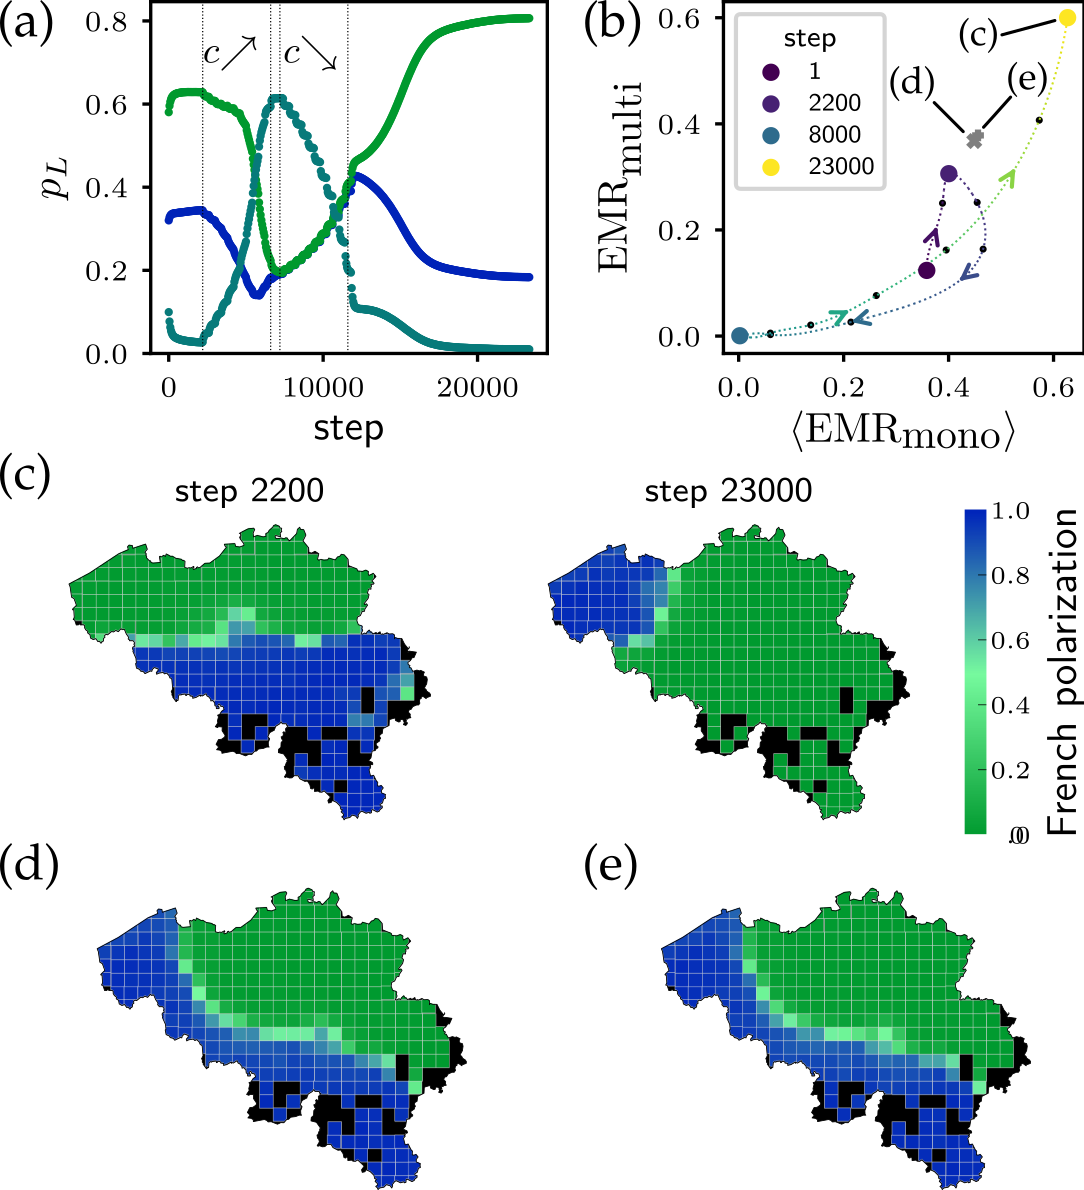
\includegraphics{varying_c_sep_to_mix_to_sep.png}
  \caption{Evolution of the state of the metapopulation model in Belgium when $c$
  varies, first slowly increased and then decreased to recover the original value. We
  fixed $s=q=1/2$ and $\mu=0.02$. (a) Evolution of the global proportions $p_L$ of
  individuals belonging to each $L$-group. The blue curve corresponds to French
  monolinguals, light green to Dutch monolinguals and dark green to bilinguals. (b)
  Trajectory of the system in the \ac{EMR} space: on the $x$-axis the average of the
  \ac{EMR} between each monolingual community and the whole population, and on the
  $y$-axis the one between bilinguals and the whole population. The initial state and
  the stable states the system went through are marked by coloured circles, while
  black ones mark additional points where the \ac{EMR} was calculated, and the dashed
  line the interpolation between them. (c) Polarisation maps of French in the initial
  and final states, both featuring a boundary but located in different areas, thus
  showing the irreversibility of the dynamics. (d)-(e) Polarisation maps of French in
  the final states of simulations including transborder commuters from France and the
  Netherlands, respectively with proportions $p_{\text{TB}}$ equal to $0.5\%$ and
  $0.2\%$ of the population of the border municipalities of these two countries. The
  points in the \ac{EMR} space corresponding to these final states are also
  represented in panel (b).}
  \label{fig:varying_c_sep_to_mix_to_sep}
\end{figure}
    
The effect of multilingual education or, in general, policies favouring the use of one
or several languages can alter the values of our model parameters. For example, $c$
represents how monolinguals learn the other language. This process can be facilitated by
the similarity between the languages or by teaching in both languages at school, for
instance. Next, we investigate whether a parameter changing in time can perturb the
system out of a stable state, and how the transition to a completely different
configuration occurs. To this end, we run a simulation for 23000 steps and present the
results in \cref{fig:varying_c_sep_to_mix_to_sep}. To explore the effects of the $c$
parameter evolution alone, we fix the other parameters $s = q = 1/2$ and $\mu = 0.02$.
We start from our initial conditions with $c = 0.005$, which converges to a stable state
with a boundary (see the first map of \cref{fig:varying_c_sep_to_mix_to_sep}(c)). After
2200 steps, we then increase $c$ by $0.005$ every $400$ steps until we reach $c =
0.055$. The system converges quickly to a state of mixed coexistence, with a majority of
bilinguals and equal proportions of monolinguals, like in
\cref{fig:single_to_metapop_BE}(e). $c$ is then decreased at the same rate as before to
reach its initial value of $0.005$. The system eventually converges to a state
displaying a boundary, but displaced compared to its initial position. The resulting
trajectory in the \ac{EMR} space in \cref{fig:varying_c_sep_to_mix_to_sep}(b) shows that
the final stable state exhibits more segregation for both monolinguals and bilinguals,
since the boundary between communities lies in the countryside, and not around Brussels
as in the original scenario. The importance of the history of languages is hence clearly
shown by this experiment.

The seemingly random placement of the boundary may be owed to the absence of constraints
on the system, which is completely closed. In reality a country is an open system with
exterior influences, notably from its direct neighbours. Thus, we ran the same
simulation with transborder proportions $p_{\text{TB}}$ equal to $0.5\%$ and $0.2\%$ of
the population of the border municipalities of France and the Netherlands commuting to
Belgium. We use the population censuses of these two countries at a municipality
level\footnote{Available at \url{https://www.insee.fr/fr/statistiques/4989724} for
France and at
\url{https://opendata.cbs.nl/statline/\#/CBS/nl/dataset/70072ned/table?dl=3B993} for the
Netherlands.} to determine how many commuters will come from each municipality close to
the border. On each side of the two borders, we only keep cells and municipalities
located less than \SI{50}{\kilo \meter} away from the border. We take a fixed proportion
$p_{\text{TB}}$ of the population of each of these municipalities as our transborder
commuters. Then, to spread the commuters of each municipality to the cells in Belgium,
we use a very simple gravity law \cite{SenGravityModels1995}, stating that the number of
commuters going from municipality $\gamma$ to cell $j$ is such that
\begin{equation}
  T_{\gamma j} \propto \frac{P_\gamma P_j}{d_{\gamma j}^2},
\end{equation}
with $P$ denoting the population and $d$ the inter-centroid distance. The normalisation
for every $\gamma$ is given by
\begin{equation}
  \sum_{j \in \mathcal{B}} T_{\gamma j} = p_{\text{TB}} P_\gamma,
\end{equation}
with $\mathcal{B}$ the set of border cells. These commuters $T_{\gamma j}$ then
appear as an additional fixed population of monolinguals at every work step in the cell
$j$. These boundary conditions stabilize the final state of convergence, as the
linguistic boundary resulting from the process of varying $c$ is similar for the two
values of $p_{\text{TB}}$, following the orientation of the two opposite borders (see
\cref{fig:varying_c_sep_to_mix_to_sep}(d-e)). This positioning is a clear improvement
over the closed-system simulation, albeit still not quite the one we observed in
\cref{fig:cat_be_maps}. In \cref{fig:varying_c_sep_to_mix_to_sep}(b), the positions of
these two states in the \ac{EMR} space are also shown to be much closer to the original
state than the final state of the first trajectory.

More complex settings could be contemplated to get closer to a realistic solution. A
space-dependent prestige could be introduced, taking different values in Flanders,
Wallonia and Brussels for instance. Also, we here considered only the commuting part of
human mobility, but other kinds of mobility like migrations may have their importance.
This is especially true for attractive metropolises like Brussels, which are typically
places of intense language contact \cite{SimonCitiesTranslation2011}. However, in this
simulation the aim was to check the irreversibility of a change when increasing the ease
to learn the other language and subsequently decreasing it to its original value, which
was indeed confirmed. 



\section{Discussion}
\label{sec:multiling_discussion}
This chapter has presented our exploration of the spatial distribution patterns of
language competition and coexistence in multilingual societies. It consisted in first
introducing the \ac{EMR}, a metric capable of measuring the spatial
segregation of a group in a given society, starting from a distance between its
distribution and that of the whole population. Two main configurations have thus been
observed: either spatial mixing with multilinguals widespread, or separate linguistic
groups with a clear boundary between them and multilinguals concentrating around it. 

Despite the ubiquity of these two configurations and their apparent temporal stability,
the models introduced in the literature were not able to offer clear solutions capturing
them. As we show, the main difficulty comes from the role of bilinguals in keeping
languages alive. In many occasions, the monolingual community of one of the languages
may become virtually extinct, and its use relies only on the bilingual group. We have
introduced a model taking this into account and have shown that it is able to produce
naturally both configurations as stable solutions without the need for artificial
non-linearities. The model features a parameter considering the preference of bilinguals
for one of the two languages. This preference actually acts as a kind of defence
mechanism since the use by bilinguals of the endangered language may be enough to save
it, countering a possibly lower prestige of the language within society as a whole. The
ease to learn the other language also has a role in the model. It may be influenced by
both the similarity between languages, which can hardly be controlled, but also by the
policies put into place to facilitate its learning. We have shown that this parameter is
critical to determine whether languages can coexist. The parameters of the model could
be estimated using longitudinal data. The scope of this work was not predictive, but
rather to study stable solutions of the model, so we leave it here for future work.

When spatial interactions are taken into account via the commuting patterns of
individuals, the model is able to reach a stable state where two language communities
are separated by a boundary around which they coexist. In this case, however, we have
shown that, quite counter-intuitively, increasing this ease to learn the other language
may break the existing boundary and lead to extinction, and not to the desired
coexistence with mixing of the languages. This calls for caution when designing policies
since the final state is strongly history-dependent.

Overall, our findings shed light on the role of heterogeneous speech communities in
multilingual societies, and they may help shape the objectives and nature of language
planning \cite{KaplanLanguagePlanning1997} in many countries where accelerated changes
are threatening cultural diversity.


\end{document}
